\documentclass[10pt]{beamer}

% ------------------------------------------------------------------------
% Carga de tu preámbulo personalizado (preamble.tex).
% Asegúrate de tenerlo en la misma carpeta para que \input funcione.
% ------------------------------------------------------------------------
\usetheme[progressbar=frametitle]{metropolis}
\usepackage{appendixnumberbeamer}
\usepackage{fancyvrb}
\usepackage{booktabs}
\usepackage[scale=2]{ccicons}
\usepackage{pgfplots}
\usepgfplotslibrary{dateplot}
\usepackage{type1cm}
\usepackage{lettrine}
\usepackage{ragged2e}
\usepackage{xspace}
\newcommand{\themename}{\textbf{\textsc{metropolis}}\xspace}
\usepackage{graphicx} % Allows including images
\usepackage{booktabs} % Allows the use of \toprule, \midrule and \bottomrule in tables
\usepackage[utf8]{inputenc} %solucion del problema de los acentos.
\usepackage{xcolor}
\definecolor{LightGray}{gray}{0.9}

\usepackage{minted}
\usemintedstyle{tango}
\newcommand{\mypyfile}[1]{\inputminted[linenos=true, fontsize=\footnotesize, frame=lines, framesep=5\fboxrule,framerule=1pt]{python}{#1}}

\setminted[python]{breaklines,frame=lines,framesep=2mm,baselinestretch=1.2,bgcolor=LightGray,linenos, fontsize=\footnotesize} % obeytabs=true, tabsize=2, showtabs=true}

%%%%%%%%%%%%%%%%%%%%%%%%%%%%%%%%%%%%%%%%%%%%%%%%%%%%%%%%%%%%%%%%%%%%%%%%%%%%%%%%%%%%%%
\setbeamercolor{progress bar}{fg=blue!50!black,bg=white!50!black}
\setbeamercolor{title separator}{fg=red!50!black,bg=white!50!black}
\setbeamercolor{frametitle}{fg=white!80!black,bg=red!50!black}
\title[PCFI161]{Programaci\'on para F\'isica y Astronom\'ia}
\subtitle{Departamento de Física.}

\newcommand{\myfront}{
\author[PCFI161]{Corodinadora: C Loyola \\ Profesoras/es C Loyola / C Femenías / Y Navarrete / C Ruiz}
\institute[UNAB]{Universidad Andrés Bello}
\date{Primer Semestre 2025}
}

\titlegraphic{%
  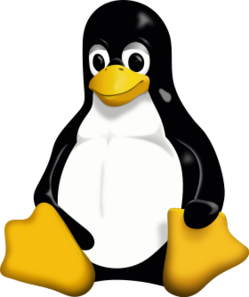
\includegraphics[width=.08\textwidth]{logo-tux.png}\hfill
  
\includegraphics[width=.3\textwidth]{logo-unab.png}\hfill
  
\includegraphics[width=.08\textwidth]{logo-python.png}
}

\makeatletter
\setbeamertemplate{title page}{
  \begin{minipage}[b][\paperheight]{\textwidth}
    \vfill%
    \ifx\inserttitle\@empty\else\usebeamertemplate*{title}\fi
    \ifx\insertsubtitle\@empty\else\usebeamertemplate*{subtitle}\fi
    \usebeamertemplate*{title separator}
    \ifx\beamer@shortauthor\@empty\else\usebeamertemplate*{author}\fi
    \ifx\insertdate\@empty\else\usebeamertemplate*{date}\fi
    \ifx\insertinstitute\@empty\else\usebeamertemplate*{institute}\fi
    \vfill
    \ifx\inserttitlegraphic\@empty\else\inserttitlegraphic\fi
    \vspace*{1cm}
  \end{minipage}
}
\makeatother


\makeatletter
\setlength{\metropolis@titleseparator@linewidth}{2pt}
\setlength{\metropolis@progressonsectionpage@linewidth}{2pt}
\setlength{\metropolis@progressinheadfoot@linewidth}{2pt}
\makeatother


\begin{document}

% ------------------------------------------------------------------------
% Portada de la Presentación
% ------------------------------------------------------------------------
\myfront{}

% ------------------------------------------------------------------------
% Slide 1: Título de la Sesión
% ------------------------------------------------------------------------
\begin{frame}
  \titlepage
  % Por ejemplo:
  % \title{Semana 8 - Sesión 1 (Sesión 15): Clases y Análisis de Datos Básico}
\end{frame}

% ------------------------------------------------------------------------
% Slide 2: Índice / Tabla de Contenidos
% ------------------------------------------------------------------------
\begin{frame}
  \frametitle{Resumen - Semana 8, Sesión 1 (Sesión 15)}
  \tableofcontents
\end{frame}

% ------------------------------------------------------------------------
% Configuración de bloques
% ------------------------------------------------------------------------
\metroset{block=fill}

% ----------------------------------------------------------------------------------------
% SECCIÓN 1: Introducción y Conexión con Sesiones Previas
% ----------------------------------------------------------------------------------------
\section{Introducción y Contexto}

% ------------------------------------------------------------------------
% Slide 3: Repaso de la Semana 7
% ------------------------------------------------------------------------
\begin{frame}{Repaso de la Semana 7}
  \begin{itemize}
    \item \textbf{Semana 7, Sesión 1 (Sesión 13)}:
      \begin{itemize}
        \item Exploramos gráficos avanzados en Matplotlib (subplots múltiples, histogramas, 3D).
        \item Tuvimos un vistazo opcional a pandas para el manejo de datos tabulares.
      \end{itemize}
    \item \textbf{Semana 7, Sesión 2 (Sesión 14)}:
      \begin{itemize}
        \item Realizamos un \textbf{problema evaluado} integrando NumPy y Matplotlib (matriz aleatoria, álgebra lineal, gráficas 3D e histograma).
        \item Aclaramos dudas tras la entrega.
      \end{itemize}
    \item \textbf{Objetivo de hoy}: Iniciar \textbf{programación orientada a objetos (POO)} en Python y repasar análisis básico de datos en NumPy/pandas.
  \end{itemize}
\end{frame}

% ------------------------------------------------------------------------
% Slide 4: Objetivos de la Sesión 15
% ------------------------------------------------------------------------
\begin{frame}{Objetivos de la Sesión 15}
  \begin{itemize}
    \item \textbf{Comprender} los fundamentos de la Programación Orientada a Objetos (POO) en Python:
      \begin{itemize}
        \item Clases, objetos, atributos, métodos.
        \item Encapsulamiento básico.
      \end{itemize}
    \item \textbf{Aplicar} estos conceptos en un ejemplo sencillo (clase \texttt{Particle} o similar).
    \item \textbf{Refrescar} el uso de NumPy/pandas para análisis de datos básicos.
    \item \textbf{Ejercitar} con un problema que combine POO y datos.
  \end{itemize}
\end{frame}

% ----------------------------------------------------------------------------------------
% SECCIÓN 2: Fundamentos de Programación Orientada a Objetos en Python
% ----------------------------------------------------------------------------------------
\section{Fundamentos de POO}

% ------------------------------------------------------------------------
% Slide 5: ¿Por qué Programación Orientada a Objetos?
% ------------------------------------------------------------------------
\begin{frame}{¿Por qué POO?}
  \begin{itemize}
    \item \textbf{Organización y modularidad}: agrupa datos y métodos lógicamente.
    \item \textbf{Reutilización de código}: herencia y polimorfismo (más adelante).
    \item \textbf{Facilita} el modelado de entidades del mundo real (partículas, sistemas, objetos astronómicos).
    \item Python lo hace \textbf{fácil} con la palabra clave \texttt{class}.
  \end{itemize}
\end{frame}

% ------------------------------------------------------------------------
% Slide 6: Definición de Clases
% ------------------------------------------------------------------------
\begin{frame}[fragile]{Definición de una Clase en Python}
\begin{minted}{python}
class MiClase:
    """Docstring o descripción de la clase."""
    def __init__(self, valor):
        # Método constructor (inicializador)
        self.atributo = valor
    
    def mostrar_atributo(self):
        print("El atributo es:", self.atributo)

# Uso
obj = MiClase(10)
obj.mostrar_atributo()  # "El atributo es: 10"
\end{minted}
\begin{itemize}
  \item \textbf{self} refiere a la instancia en los métodos.
  \item \texttt{\_\_init\_\_} se llama al crear el objeto (\textbf{constructor}).
\end{itemize}
\end{frame}

% ------------------------------------------------------------------------
% Slide 7: Atributos y Métodos
% ------------------------------------------------------------------------
\begin{frame}{Atributos y Métodos}
  \begin{itemize}
    \item \textbf{Atributos} (variables) caracterizan el estado de un objeto.
      \begin{itemize}
        \item Definidos en \texttt{\_\_init\_\_} o fuera (variables de clase).
      \end{itemize}
    \item \textbf{Métodos} (funciones) definen el comportamiento.
      \begin{itemize}
        \item \textbf{Instancia}: necesitan \texttt{self}.
        \item \textbf{Clase}: usan \texttt{@classmethod} y tienen \texttt{cls} en lugar de \texttt{self}.
        \item \textbf{Estáticos}: usan \texttt{@staticmethod} y no reciben \texttt{self} ni \texttt{cls}.
      \end{itemize}
    \item Encapsulamiento es \textbf{limitado} en Python (no hay private real), pero se puede usar guión bajo (\texttt{\_atributo}) para indicar uso interno.
  \end{itemize}
\end{frame}

% ------------------------------------------------------------------------
% Slide 8: Ejemplo: Clase \texttt{Particle}
% ------------------------------------------------------------------------
\begin{frame}[fragile]{Ejemplo: Clase Particle}
\begin{minted}{python}
import math

class Particle:
    def __init__(self, mass, x, y, vx, vy):
        self.mass = mass
        self.x = x
        self.y = y
        self.vx = vx
        self.vy = vy
    
    def kinetic_energy(self):
        """Retorna la energía cinética de la partícula."""
        v2 = self.vx**2 + self.vy**2
        return 0.5 * self.mass * v2
    
    def distance(self, other):
        """Distancia a otra partícula."""
        dx = self.x - other.x
        dy = self.y - other.y
        return math.sqrt(dx**2 + dy**2)
\end{minted}
\end{frame}

% ------------------------------------------------------------------------
% Slide 9: Uso de la Clase \texttt{Particle}
% ------------------------------------------------------------------------
\begin{frame}[fragile]{Uso y Ejemplo}
\begin{minted}{python}
p1 = Particle(mass=2.0, x=0, y=0, vx=3, vy=4)
p2 = Particle(mass=1.5, x=5, y=5, vx=0, vy=-2)

print("E_c de p1:", p1.kinetic_energy())  # 0.5*2*25 = 25
dist = p1.distance(p2)
print("Distancia p1 - p2:", dist)
\end{minted}
\begin{itemize}
  \item Se pueden crear múltiples partículas y realizar cálculos \textbf{similares} sin reescribir la lógica.
  \item Facilita la \textbf{extensión} futura (métodos de colisiones, etc.).
\end{itemize}
\end{frame}

% ----------------------------------------------------------------------------------------
% SECCIÓN 3: Análisis de Datos con NumPy/Pandas (Repaso)
% ----------------------------------------------------------------------------------------
\section{Análisis de Datos Rápido}

% ------------------------------------------------------------------------
% Slide 10: Llamado a Pandas
% ------------------------------------------------------------------------
\begin{frame}[fragile]{Recordatorio de Pandas}
\begin{minted}{python}
import pandas as pd

df = pd.read_csv("datos_simulacion.csv")
print(df.head())
print(df.describe())

# Seleccionar columna "VelX"
velx = df["VelX"]
# Calcular promedio de VelX
prom_velx = velx.mean()
print("Promedio de VelX:", prom_velx)
\end{minted}
\begin{itemize}
  \item \textbf{df.head()} muestra las primeras filas.
  \item \textbf{df.describe()} da estadísticas (count, mean, std, min, max, quartiles).
\end{itemize}
\end{frame}

% ------------------------------------------------------------------------
% Slide 11: Conexión con POO
% ------------------------------------------------------------------------
\begin{frame}{Unir POO y Pandas}
  \begin{itemize}
    \item \textbf{Ejemplo}:
      \begin{itemize}
        \item Cargar datos de partículas (\texttt{mass, x, y, vx, vy}).
        \item Crear objetos \texttt{Particle} a partir de cada fila del DataFrame.
        \item Calcular energía cinética total, distancias, etc.
      \end{itemize}
    \item Nos ayuda a \textbf{organizar} simulaciones más complejas.
  \end{itemize}
\end{frame}

% ----------------------------------------------------------------------------------------
% SECCIÓN 4: Ejercicios Prácticos
% ----------------------------------------------------------------------------------------
\section{Ejercicios Prácticos}

% ------------------------------------------------------------------------
% Slide 12: Ejercicio 1 - Clase Sencilla
% ------------------------------------------------------------------------
\begin{frame}{Ejercicio 1: Clase para Administrar Notas de Estudiantes}
  \begin{block}{Enunciado}
    \begin{itemize}
      \item Crear una clase \textbf{Student} con atributos: \(\texttt{name}\), \(\texttt{grades}\) (lista o array).
      \item Método \texttt{average()} que retorne el promedio de \texttt{grades}.
      \item Método \texttt{show\_info()} que imprima nombre y promedio.
      \item Instanciar varios objetos y mostrarlos en un \textbf{DataFrame de pandas} (opcional).
    \end{itemize}
  \end{block}
  \textbf{Sugerencia}: Manejar notas como lista de floats y \textbf{numpy.mean} u operaciones directas.
\end{frame}

% ------------------------------------------------------------------------
% Slide 13: Ejercicio 2 - Partículas desde CSV
% ------------------------------------------------------------------------
\begin{frame}{Ejercicio 2: Partículas desde CSV (pandas + POO)}
  \begin{block}{Enunciado}
    \begin{itemize}
      \item Suponer un archivo \(\texttt{particles.csv}\) con columnas: \(\texttt{mass, x, y, vx, vy}\).
      \item Cargarlo con \texttt{pandas}.
      \item Por cada fila, crear un objeto \texttt{Particle}.
      \item Calcular la \textbf{energía cinética total} y la \textbf{posición promedio} (\((\bar{x}, \bar{y})\)).
      \item (Opcional) Graficar las partículas en un scatter (\texttt{x} vs \texttt{y}) usando \textbf{Matplotlib}.
    \end{itemize}
  \end{block}
  \textbf{Objetivo}: Combinar la \textbf{clase Particle} con datos reales/leídos de un CSV.
\end{frame}

% ------------------------------------------------------------------------
% Slide 14: Ejercicio 3 - Cálculo de Distancias
% ------------------------------------------------------------------------
\begin{frame}{Ejercicio 3: Matriz de Distancias con NumPy}
  \begin{block}{Enunciado}
    \begin{itemize}
      \item Teniendo \texttt{n} partículas (ya sea generadas o leídas):
      \item Crear una \textbf{matriz NxN} donde la entrada \((i,j)\) sea la distancia entre partícula \(i\) y \(j\).
      \item Usar preferentemente \textbf{NumPy} para vectorizar o, si no, hacerlo en un doble \textbf{for}.
      \item (Opcional) Mostrarla como un \textbf{mapa de calor} con \texttt{plt.imshow}.
    \end{itemize}
  \end{block}
  \textbf{Sugerencia}: \textbf{p1.distance(p2)} es el método que definimos en la clase \texttt{Particle}.
\end{frame}

% ------------------------------------------------------------------------
% Slide 15: Trabajo en Grupos
% ------------------------------------------------------------------------
\begin{frame}{Trabajo en Grupos}
  \begin{itemize}
    \item Formar \textbf{parejas/tríos}.
    \item Seleccionar al menos \textbf{2 ejercicios} anteriores (o crear una fusión).
    \item Implementar soluciones en un \textbf{notebook} de Colab.
    \item Agregar \textbf{gráficas}, \textbf{comentarios} y \textbf{pruebas} de cada parte.
    \item Comparar resultados y dudas al final.
  \end{itemize}
\end{frame}

% ------------------------------------------------------------------------
% Slide 16: Sugerencias Generales
% ------------------------------------------------------------------------
\begin{frame}{Sugerencias Generales}
  \begin{itemize}
    \item \textbf{POO}: mantén las clases simples y bien comentadas.
    \item \textbf{pandas}: \texttt{df.iterrows()} o \texttt{df.itertuples()} puede ayudarte a iterar filas.
    \item \textbf{NumPy}: para la matriz de distancias, considera \texttt{np.zeros((n,n))} de base.
    \item \textbf{Visualización}: usa \(\texttt{plt.scatter(df['x'], df['y'])}\) si usas DataFrame.
  \end{itemize}
\end{frame}

% ------------------------------------------------------------------------
% Slide 17: Espacio para Dudas
% ------------------------------------------------------------------------
\begin{frame}{Espacio para Dudas}
  \begin{itemize}
    \item ¿Dificultades al instanciar objetos desde DataFrame?
    \item ¿Uso de \textbf{NumPy} en la creación de la matriz de distancias?
    \item ¿Cómo mostrar la información en un \textbf{DataFrame} de forma clara?
    \item \textbf{Preguntar abiertamente} si algo no está claro.
  \end{itemize}
\end{frame}

% ----------------------------------------------------------------------------------------
% SECCIÓN 5: Conclusiones y Próximos Pasos
% ----------------------------------------------------------------------------------------
\section{Conclusiones y Próximos Pasos}

% ------------------------------------------------------------------------
% Slide 18: Discusión de Soluciones
% ------------------------------------------------------------------------
\begin{frame}{Discusión de Soluciones}
  \begin{itemize}
    \item Comparte \textbf{cómo implementaste} la clase y las funciones.
    \item Menciona si \textbf{pandas} facilitó la lectura de datos.
    \item Para la matriz de distancias, ¿usaste \textbf{doble for} o intentaste algo vectorizado?
    \item Resultados numéricos y/o visuales (\textbf{gráficas}) que surgieron.
  \end{itemize}
\end{frame}

% ------------------------------------------------------------------------
% Slide 19: Conclusiones de la Sesión 15
% ------------------------------------------------------------------------
\begin{frame}{Conclusiones de la Sesión 15}
  \begin{itemize}
    \item Iniciamos la \textbf{Programación Orientada a Objetos} (POO) en Python.
      \begin{itemize}
        \item Clases, atributos, métodos, constructor.
        \item Ejemplo con \texttt{Particle} y distancias.
      \end{itemize}
    \item Reforzamos la \textbf{integración} con \textbf{NumPy} y \textbf{pandas}, importante para \textbf{análisis de datos} y simulaciones.
    \item Seguiremos expandiendo POO y su aplicación en futuros problemas más complejos.
  \end{itemize}
\end{frame}

% ------------------------------------------------------------------------
% Slide 20: Próxima Sesión
% ------------------------------------------------------------------------
\begin{frame}{Próximos Temas (Semana 8, Sesión 2)}
  \begin{itemize}
    \item Continuar con \textbf{POO} (herencia, métodos especiales).
    \item Ejemplos avanzados: \textbf{clases para manejo estadístico}, o \textbf{modelos de partículas} con interacciones básicas.
    \item Se revisará la \textbf{retroalimentación} del problema evaluado de la semana pasada.
  \end{itemize}
  \vspace{0.3cm}
  \textbf{Recomendación}: Repasar la sintaxis de \texttt{class} y crear ejemplos propios para consolidar POO.
\end{frame}

% ------------------------------------------------------------------------
% Slide 21: Recursos Adicionales
% ------------------------------------------------------------------------
\begin{frame}{Recursos Adicionales}
  \begin{itemize}
    \item \href{https://docs.python.org/3/tutorial/classes.html}{\textbf{Python Tutorial - Classes}} (documentación oficial).
    \item \href{https://pandas.pydata.org/}{\textbf{Pandas Documentation}} para operaciones de DataFrame.
    \item \href{https://realpython.com/}{\textbf{Real Python}} - guías sobre OOP y análisis de datos en Python.
    \item \href{https://numpy.org/doc/stable/reference/routines.linalg.html}{\textbf{NumPy linalg}} - recordatorio de funciones.
  \end{itemize}
\end{frame}

% ------------------------------------------------------------------------
% Slide 22: Cierre de la Sesión
% ------------------------------------------------------------------------
\begin{frame}
  \Huge{\centerline{¡Gracias y hasta la próxima sesión!}}
  \vspace{0.4cm}
  \normalsize
  \begin{itemize}
    \item Practiquen la creación de \textbf{clases} y la \textbf{lectura} de datos con \textbf{pandas}.
    \item ¡Nos vemos en la \textbf{Semana 8, Sesión 2} para profundizar POO!
  \end{itemize}
\end{frame}

\end{document}

